\label{sec:yields}
After the selections described in Section \ref{sec:event_selection}, the event yields are extracted for signal and backgrounds for each of the four periods of Run2, for the signal and control regions.

\subsection{Four lepton channel}
The pre-fit yields for the signal and background processes for the signal region
with four leptons passing the tight selection and a photon passing the cut-based ID (SR4P\_1P),
can be seen in Table \ref{tab:Run2_SR4P_phoCR_lepCR}.
Additional tables, including also the observed number of data events, are provided
for the fake photon application region (Table \ref{tab:yields_Run2_CR4P_1F_lepCR}),
and for the fake lepton application regions (Tables \ref{tab:yields_Run2_CR3P1F_1P} and \ref{tab:yields_Run2_CR2P2F_1P}).

\begin{table}
\caption{Yields from the signal region SR4P\_1P, with four leptons passing the tight selection and a photon passing the cut-based ID.}
\label{tab:Run2_SR4P_phoCR_lepCR}
% Note: this is from the variable mZZGloose
\resizebox{\textwidth}{!}{%
\begin{tabular}{lrrrrr}
\toprule
{} & \multicolumn{1}{c}{2016preVFP} & \multicolumn{1}{c}{2016postVFP} & \multicolumn{1}{c}{2017} & \multicolumn{1}{c}{2018} & \multicolumn{1}{c}{Run2} \\
\midrule
ZZGTo4LG-prompt  &  1.889 $\pm$ 0.046 &  1.657 $\pm$ 0.040 &  3.812 $\pm$ 0.097 &   5.480 $\pm$ 0.137 &  12.838 $\pm$ 0.178 \\
ZZTo4l-prompt    &  1.185 $\pm$ 0.023 &  1.093 $\pm$ 0.021 &  2.559 $\pm$ 0.036 &   3.710 $\pm$ 0.052 &   8.546 $\pm$ 0.071 \\
ggTo4e-prompt    &  0.030 $\pm$ 0.001 &  0.029 $\pm$ 0.001 &  0.072 $\pm$ 0.002 &   0.101 $\pm$ 0.003 &   0.232 $\pm$ 0.004 \\
ggTo2e2mu-prompt &  0.062 $\pm$ 0.003 &  0.056 $\pm$ 0.002 &  0.066 $\pm$ 0.003 &   0.102 $\pm$ 0.004 &   0.286 $\pm$ 0.006 \\
ggTo4mu-prompt   &  0.056 $\pm$ 0.001 &  0.046 $\pm$ 0.001 &  0.113 $\pm$ 0.003 &   0.153 $\pm$ 0.004 &   0.368 $\pm$ 0.005 \\
ZZZ-prompt       &  0.007 $\pm$ 0.005 &  0.000 $\pm$ 0.000 &  0.017 $\pm$ 0.008 &   0.029 $\pm$ 0.010 &   0.053 $\pm$ 0.014 \\
TTZJets-prompt   &  0.010 $\pm$ 0.002 &  0.009 $\pm$ 0.002 &  0.034 $\pm$ 0.005 &   0.040 $\pm$ 0.006 &   0.094 $\pm$ 0.008 \\
fake\_photons     &  1.212 $\pm$ 0.638 &  0.710 $\pm$ 0.411 &  1.195 $\pm$ 0.489 &   1.736 $\pm$ 0.588 &   4.853 $\pm$ 1.077 \\
WZZ-prompt       &  0.000 $\pm$ 0.000 &  0.014 $\pm$ 0.010 &  0.017 $\pm$ 0.016 &   0.053 $\pm$ 0.024 &   0.085 $\pm$ 0.031 \\
WWZ-prompt       &  0.000 $\pm$ 0.000 &  0.040 $\pm$ 0.040 &  0.041 $\pm$ 0.041 &   0.082 $\pm$ 0.058 &   0.163 $\pm$ 0.081 \\
\midrule
Total            &  4.451 $\pm$ 0.640 &  3.653 $\pm$ 0.415 &  7.927 $\pm$ 0.502 &  11.485 $\pm$ 0.609 &  27.517 $\pm$ 1.098 \\
\bottomrule
\end{tabular}
}
\end{table}

\begin{table}
\caption{Yields from the fake photon application region CR4P\_1F, with four leptons passing the tight selection and a photon passing the VeryLoose ID but failing the cut-based ID Loose.}
\label{tab:yields_Run2_CR4P_1F_lepCR}
\resizebox{\textwidth}{!}{%
\begin{tabular}{lrrrrr}
\toprule
{} & \multicolumn{1}{c}{2016preVFP} & \multicolumn{1}{c}{2016postVFP} & \multicolumn{1}{c}{2017} & \multicolumn{1}{c}{2018} & \multicolumn{1}{c}{Run2} \\
\midrule
ZZGTo4LG  &  0.286 $\pm$ 0.019 &  0.270 $\pm$ 0.016 &  0.751 $\pm$ 0.044 &   1.061 $\pm$ 0.060 &   2.367 $\pm$ 0.078 \\
ZZTo4l    &  2.270 $\pm$ 0.032 &  2.162 $\pm$ 0.029 &  6.228 $\pm$ 0.057 &   9.118 $\pm$ 0.082 &  19.777 $\pm$ 0.108 \\
ggTo4e    &  0.050 $\pm$ 0.001 &  0.048 $\pm$ 0.001 &  0.137 $\pm$ 0.003 &   0.203 $\pm$ 0.004 &   0.438 $\pm$ 0.005 \\
ggTo2e2mu &  0.131 $\pm$ 0.004 &  0.128 $\pm$ 0.004 &  0.180 $\pm$ 0.005 &   0.253 $\pm$ 0.007 &   0.691 $\pm$ 0.010 \\
ggTo4mu   &  0.088 $\pm$ 0.002 &  0.075 $\pm$ 0.001 &  0.202 $\pm$ 0.004 &   0.305 $\pm$ 0.006 &   0.671 $\pm$ 0.007 \\
ZZZ       &  0.039 $\pm$ 0.011 &  0.018 $\pm$ 0.009 &  0.057 $\pm$ 0.015 &   0.066 $\pm$ 0.018 &   0.180 $\pm$ 0.027 \\
WZZ       &  0.051 $\pm$ 0.020 &  0.051 $\pm$ 0.019 &  0.077 $\pm$ 0.028 &   0.120 $\pm$ 0.038 &   0.299 $\pm$ 0.055 \\
WWZ       &  0.048 $\pm$ 0.048 &  0.046 $\pm$ 0.046 &  0.000 $\pm$ 0.000 &   0.000 $\pm$ 0.000 &   0.094 $\pm$ 0.067 \\
TTZJets   &  0.046 $\pm$ 0.005 &  0.039 $\pm$ 0.004 &  0.144 $\pm$ 0.010 &   0.216 $\pm$ 0.014 &   0.444 $\pm$ 0.019 \\
\midrule
Total     &  3.008 $\pm$ 0.066 &  2.836 $\pm$ 0.061 &  7.776 $\pm$ 0.079 &  11.342 $\pm$ 0.111 &  24.962 $\pm$ 0.163 \\
Data      & \multicolumn{1}{c}{4} & \multicolumn{1}{c}{3} & \multicolumn{1}{c}{6} & \multicolumn{1}{c}{9} & \multicolumn{1}{c}{22} \\
\bottomrule
\end{tabular}
}
\end{table}

\begin{table}
\caption{Yields in CR3P1F\_1P, one of the fake lepton application regions, with three leptons passing the tight selection, one passing only a loose selection, and a photon passing the cut-based ID.}
\label{tab:yields_Run2_CR3P1F_1P}
\resizebox{\textwidth}{!}{%
\begin{tabular}{lrrrrr}
\toprule
{} & \multicolumn{1}{c}{2016preVFP} & \multicolumn{1}{c}{2016postVFP} & \multicolumn{1}{c}{2017} & \multicolumn{1}{c}{2018} & \multicolumn{1}{c}{Run2} \\
\midrule
ZZGTo4LG       &  0.126 $\pm$ 0.013 &  0.131 $\pm$ 0.011 &  0.369 $\pm$ 0.031 &  0.453 $\pm$ 0.039 &  1.080 $\pm$ 0.052 \\
WZGTo3LNuG     &  0.203 $\pm$ 0.010 &  0.185 $\pm$ 0.008 &  0.392 $\pm$ 0.019 &  0.673 $\pm$ 0.030 &  1.453 $\pm$ 0.038 \\
ZGToLLG        &  0.695 $\pm$ 0.280 &  0.000 $\pm$ 0.000 &  0.463 $\pm$ 0.388 &  0.492 $\pm$ 0.447 &  1.650 $\pm$ 0.654 \\
ZZTo4l         &  0.179 $\pm$ 0.009 &  0.160 $\pm$ 0.008 &  0.412 $\pm$ 0.015 &  0.618 $\pm$ 0.021 &  1.368 $\pm$ 0.029 \\
ggTo4e         &  0.008 $\pm$ 0.000 &  0.006 $\pm$ 0.000 &  0.017 $\pm$ 0.001 &  0.029 $\pm$ 0.002 &  0.061 $\pm$ 0.002 \\
ggTo2e2mu      &  0.011 $\pm$ 0.001 &  0.009 $\pm$ 0.001 &  0.012 $\pm$ 0.001 &  0.018 $\pm$ 0.002 &  0.049 $\pm$ 0.003 \\
ggTo4mu        &  0.003 $\pm$ 0.000 &  0.002 $\pm$ 0.000 &  0.006 $\pm$ 0.001 &  0.007 $\pm$ 0.001 &  0.019 $\pm$ 0.001 \\
WZTo3LNu       &  0.359 $\pm$ 0.103 &  0.434 $\pm$ 0.093 &  0.500 $\pm$ 0.174 &  1.055 $\pm$ 0.316 &  2.348 $\pm$ 0.387 \\
ZZZ            &  0.003 $\pm$ 0.003 &  0.000 $\pm$ 0.000 &  0.010 $\pm$ 0.006 &  0.007 $\pm$ 0.005 &  0.020 $\pm$ 0.008 \\
WZZ            &  0.009 $\pm$ 0.009 &  0.000 $\pm$ 0.000 &  0.001 $\pm$ 0.012 &  0.012 $\pm$ 0.012 &  0.022 $\pm$ 0.019 \\
TTZJets        &  0.035 $\pm$ 0.004 &  0.032 $\pm$ 0.004 &  0.060 $\pm$ 0.006 &  0.107 $\pm$ 0.010 &  0.235 $\pm$ 0.013 \\
DYJetsToLL\_M50&  0.000 $\pm$ 0.000 &  0.000 $\pm$ 0.000 &  0.000 $\pm$ 0.000 &  0.680 $\pm$ 3.520 &  0.680 $\pm$ 3.520 \\
\midrule
Total          &  1.631 $\pm$ 0.299 &  0.960 $\pm$ 0.095 &  2.242 $\pm$ 0.427 &  4.152 $\pm$ 3.562 &  8.985 $\pm$ 3.602 \\
Data & \multicolumn{1}{c}{1} & \multicolumn{1}{c}{0} & \multicolumn{1}{c}{2} & \multicolumn{1}{c}{4} & \multicolumn{1}{c}{7} \\
\bottomrule
\end{tabular}
}
\end{table}

\begin{table}
\caption{Yields in CR2P2F\_1P, one of the fake lepton application regions, with two leptons passing the tight selection, two passing only a loose selection, and a photon passing the cut-based ID.}
\label{tab:yields_Run2_CR2P2F_1P}
\resizebox{\textwidth}{!}{%
\begin{tabular}{lrrrrr}
\toprule
{} & \multicolumn{1}{c}{2016preVFP} & \multicolumn{1}{c}{2016postVFP} & \multicolumn{1}{c}{2017} & \multicolumn{1}{c}{2018} & \multicolumn{1}{c}{Run2} \\
\midrule
ZZGTo4LG       &   0.008 $\pm$ 0.004 &   0.005 $\pm$ 0.002 &    0.006 $\pm$ 0.004 &    0.030 $\pm$ 0.010 &    0.050 $\pm$ 0.011 \\
WZGTo3LNuG     &   0.022 $\pm$ 0.003 &   0.019 $\pm$ 0.003 &    0.032 $\pm$ 0.005 &    0.048 $\pm$ 0.008 &    0.121 $\pm$ 0.011 \\
ZGToLLG        &   6.473 $\pm$ 0.786 &   0.000 $\pm$ 0.000 &   13.535 $\pm$ 1.451 &   20.784 $\pm$ 2.258 &   40.792 $\pm$ 2.796 \\
ZZTo4l         &   0.013 $\pm$ 0.003 &   0.011 $\pm$ 0.002 &    0.017 $\pm$ 0.003 &    0.032 $\pm$ 0.005 &    0.074 $\pm$ 0.007 \\
ggTo4e         &   0.000 $\pm$ 0.000 &   0.000 $\pm$ 0.000 &    0.000 $\pm$ 0.000 &    0.001 $\pm$ 0.000 &    0.001 $\pm$ 0.000 \\
ggTo2e2mu      &   0.000 $\pm$ 0.000 &   0.000 $\pm$ 0.000 &    0.000 $\pm$ 0.000 &    0.000 $\pm$ 0.000 &    0.001 $\pm$ 0.000 \\
WZTo3LNu       &   0.018 $\pm$ 0.035 &   0.052 $\pm$ 0.041 &    0.185 $\pm$ 0.108 &    0.238 $\pm$ 0.121 &    0.493 $\pm$ 0.171 \\
TTZJets        &   0.020 $\pm$ 0.003 &   0.017 $\pm$ 0.003 &    0.029 $\pm$ 0.004 &    0.043 $\pm$ 0.006 &    0.110 $\pm$ 0.009 \\
TZq            &   0.005 $\pm$ 0.007 &   0.000 $\pm$ 0.006 &    0.018 $\pm$ 0.009 &    0.021 $\pm$ 0.012 &    0.044 $\pm$ 0.018 \\
tW             &   0.057 $\pm$ 0.057 &   0.000 $\pm$ 0.000 &    0.088 $\pm$ 0.099 &    0.000 $\pm$ 0.000 &    0.144 $\pm$ 0.114 \\
DYJetsToLL\_M50 &   0.000 $\pm$ 0.000 &  11.019 $\pm$ 6.842 &  14.447 $\pm$ 10.750 &  29.521 $\pm$ 14.716 &  54.986 $\pm$ 19.467 \\
ggTo4mu        &   0.000 $\pm$ 0.000 &   0.000 $\pm$ 0.000 &    0.000 $\pm$ 0.000 &    0.000 $\pm$ 0.000 &    0.000 $\pm$ 0.000 \\
\midrule
Total          &   6.616 $\pm$ 0.789 &  11.123 $\pm$ 6.842 &  28.359 $\pm$ 10.849 &  50.717 $\pm$ 14.889 &  96.814 $\pm$ 19.667 \\
Data & \multicolumn{1}{c}{17} & \multicolumn{1}{c}{8} & \multicolumn{1}{c}{21} & \multicolumn{1}{c}{22} & \multicolumn{1}{c}{68} \\
\bottomrule
\end{tabular}
}
\end{table}

\begin{figure}
\subfigure [2016preVFP ] {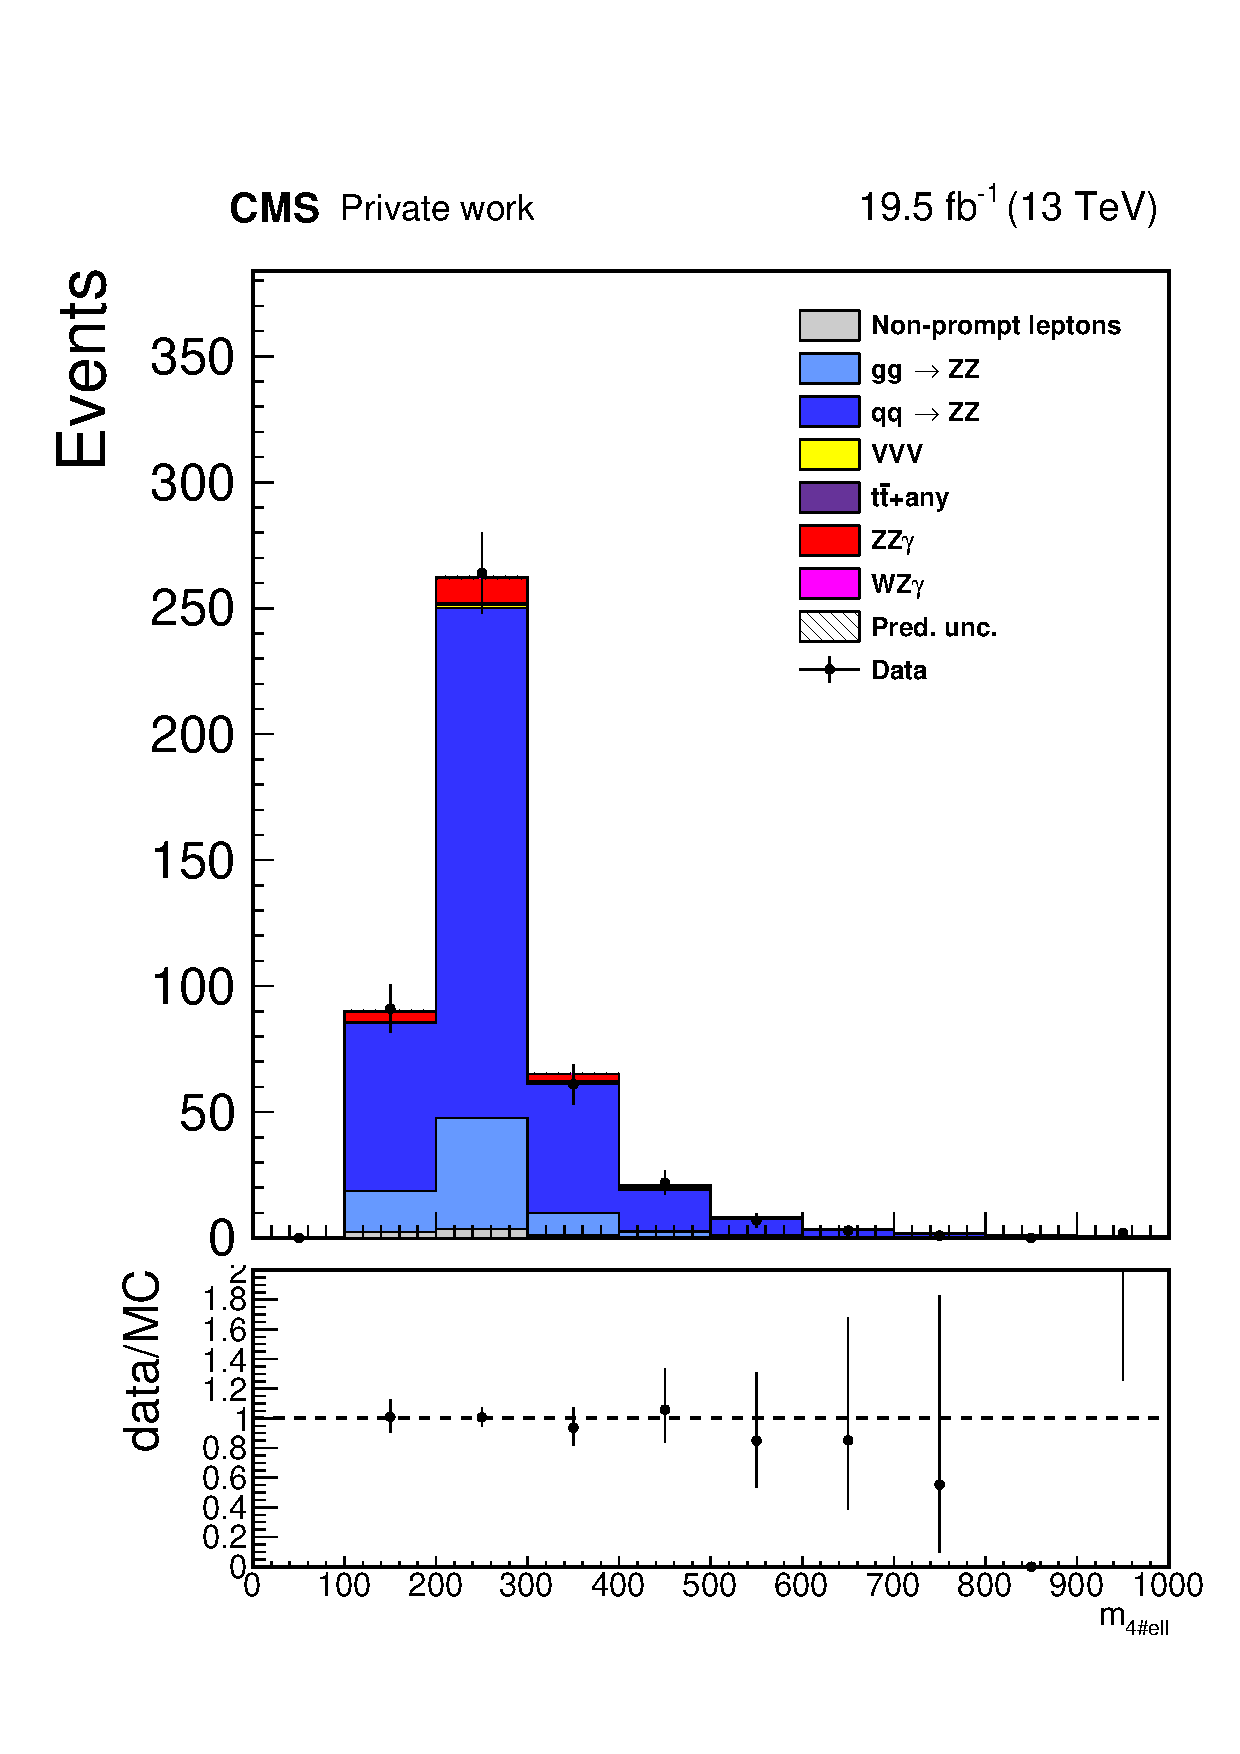
\includegraphics[width=.25\textwidth]{Figures/VVGammaAnalyzer/2016preVFP/lepCR/SR4P/ZZ_mass_pow.pdf}}%
\subfigure [2016postVFP] {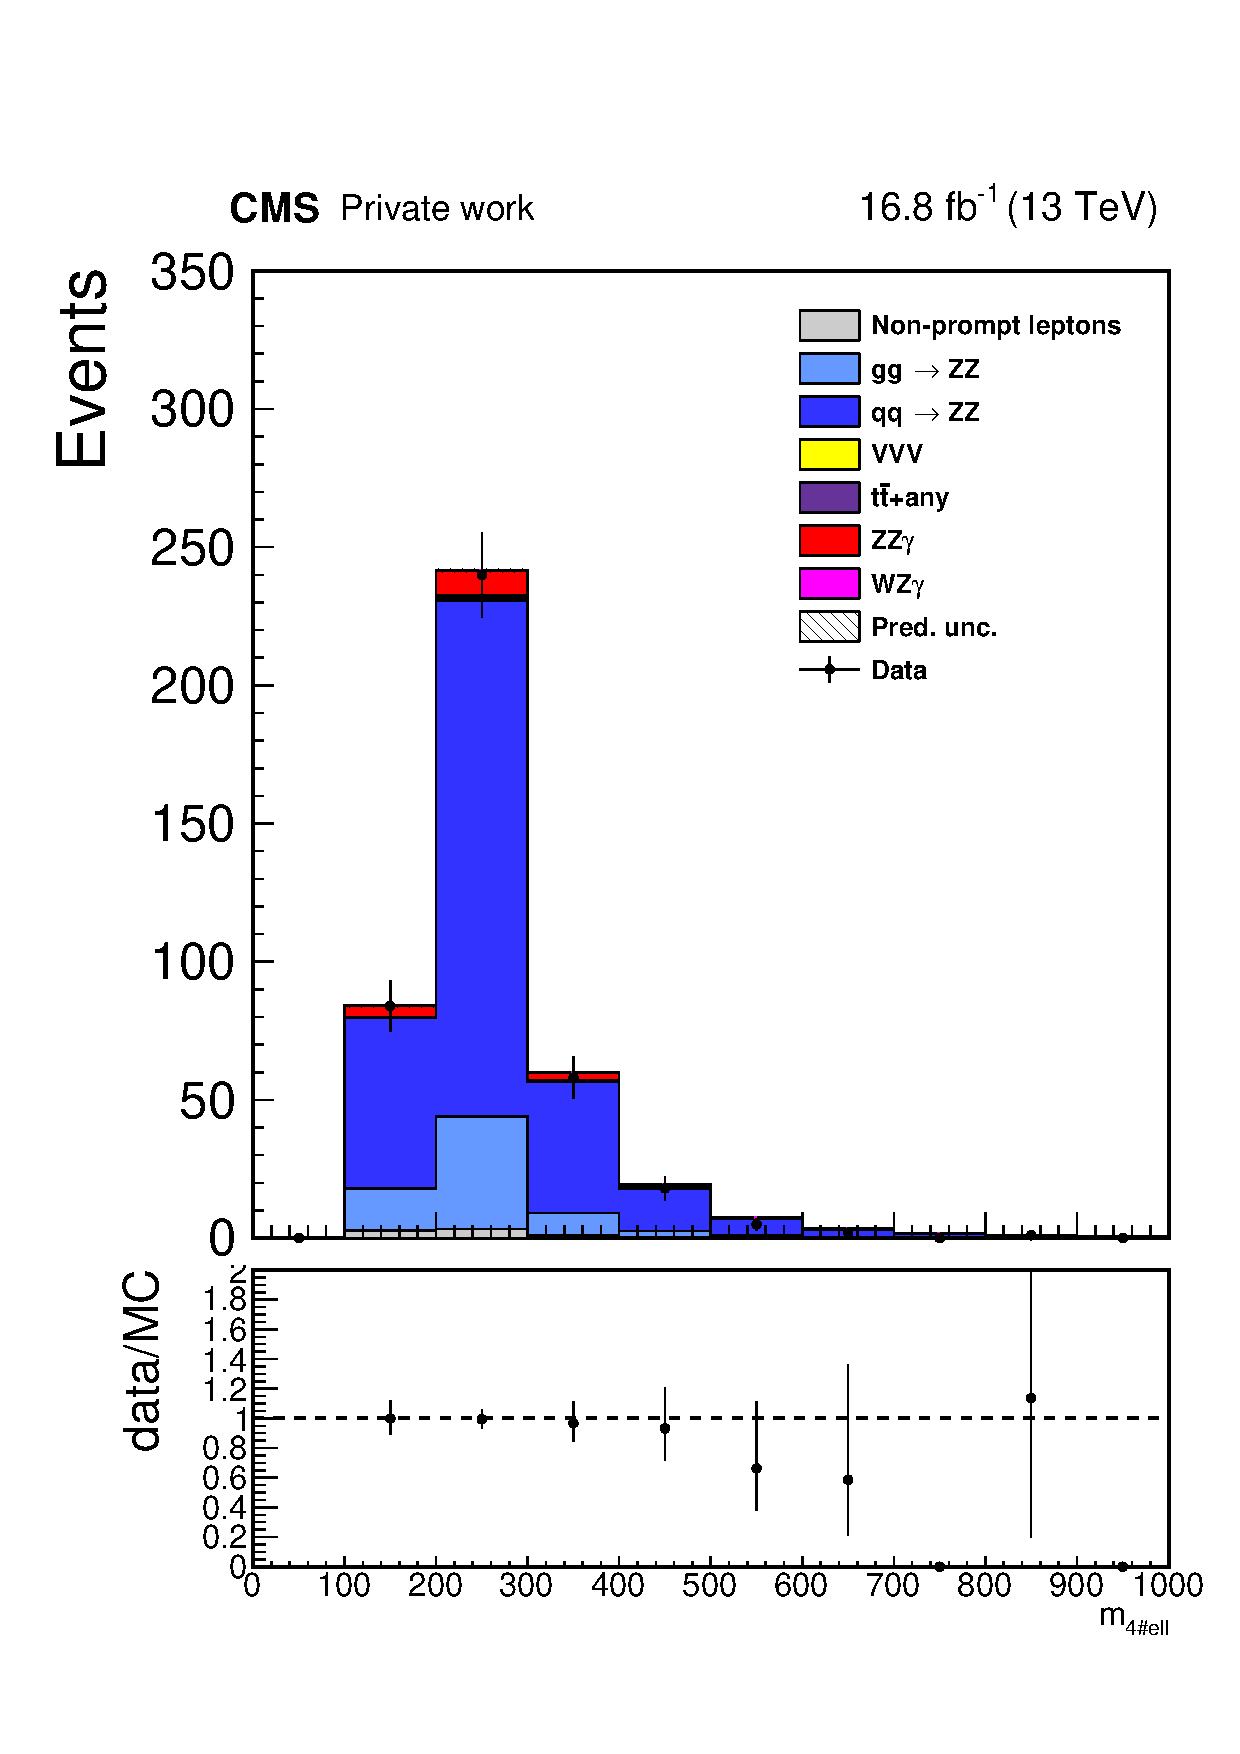
\includegraphics[width=.25\textwidth]{Figures/VVGammaAnalyzer/2016postVFP/lepCR/SR4P/ZZ_mass_pow.pdf}}%
\subfigure [2017       ] {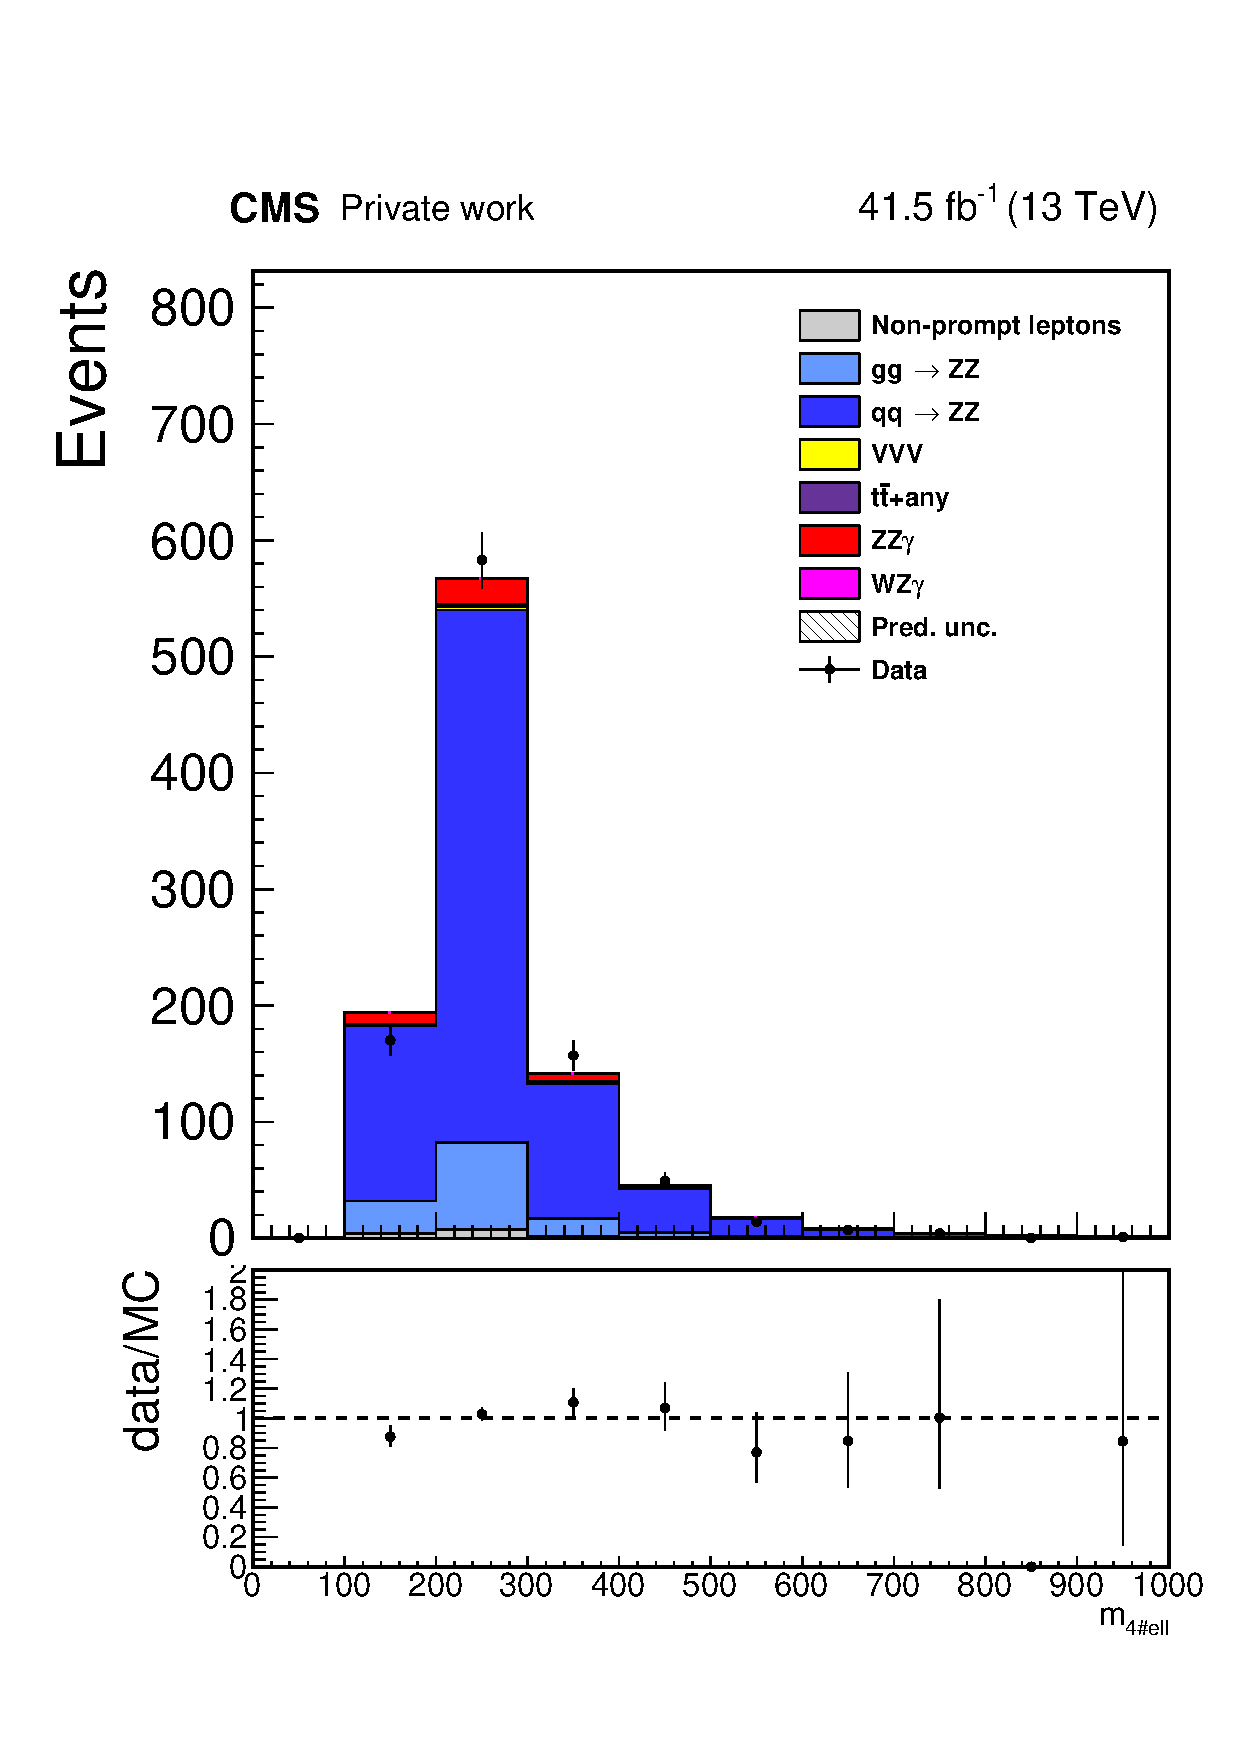
\includegraphics[width=.25\textwidth]{Figures/VVGammaAnalyzer/2017/lepCR/SR4P/ZZ_mass_pow.pdf}}%
\subfigure [2018       ] {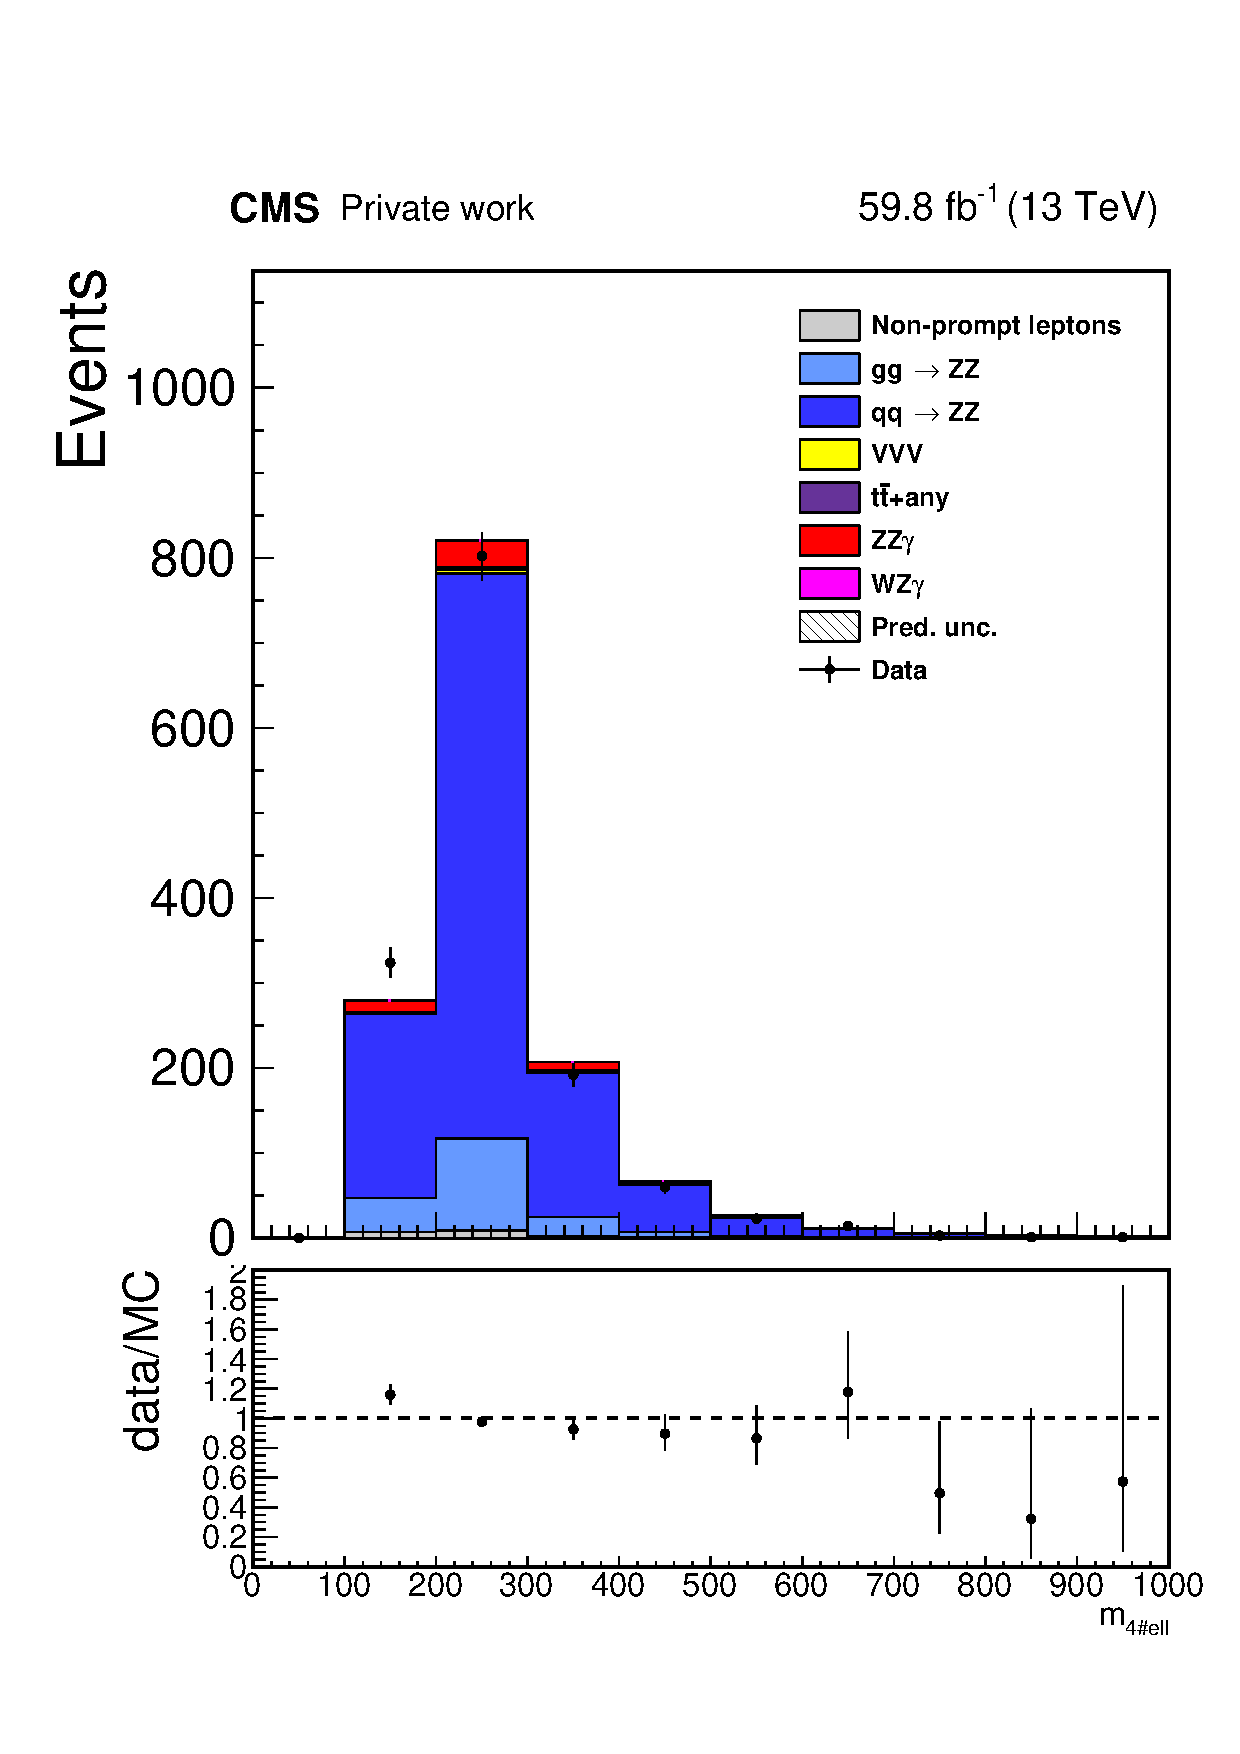
\includegraphics[width=.25\textwidth]{Figures/VVGammaAnalyzer/2018/lepCR/SR4P/ZZ_mass_pow.pdf}}
\caption{Invariant mass of the ZZ system, without any requirements on the presence of photons, for each of the data-taking periods of Run2.}
\label{fig:ZZmass_byyear}
\end{figure}
